
\section{SIGNAL MODEL DETECTOR RESPONSE TABLE}
\label{app:response_table}

In this appendix we describe digital tables which can be used to construct an accurate signal model for this analysis given any input recoil spectrum $\mathrm{d}R/\mathrm{d}E$ arising from a theoretical model. A visualization of the tables is shown in Fig.~\ref{fig:smeartable_highE}, and in section \ref{app:example_code} we show a simple example Python code of how to use the supplied tables. Currently we provide these tables only for the high-energy analysis region.

The signal model for the high-energy analysis region can be expressed analytically in the form:
%
\begin{align}
\label{eq:high2D}
  \frac{\mathrm{d} R}{\mathrm{d}\cSi} &= \int \! \frac{\mathrm{d}R}{\mathrm{d}E} \cdot \epsilon_\mathrm{S1}(\cSi) \cdot \epsilon_\mathrm{S2'}(E) \cdot p_\mathrm{S1}(\mathrm{\cSi}|E) \, \mathrm{d}E \\
  &= \int \! \frac{\mathrm{d}R}{\mathrm{d}E} G(\cSi,E) \, \mathrm{d}E
\end{align}
%
where $\epsilon_\mathrm{S1}(\cSi)$ and $\epsilon_\mathrm{S2'}(E)$ represent analysis cut efficiencies, $p_\mathrm{S1}(\mathrm{\cSi}|E)$ encodes detector effects, and $\mathrm{d}R/\mathrm{d}E$ gives the theoretically predicted nuclear recoil rate from WIMP scattering. In the second line we emphasis that all the detector and analysis effects can be encoded in a single function $G(\cSi,E)$. To make a signal prediction for the bins in our analysis, this expression needs to be integrated over the appropriate range of $\cSi$ for each bin (and divided by two to account for the banding structure in $\cSiib$):
%
\begin{equation}
  R_\mathrm{bin_i} = \frac{1}{2}\int_{\mathrm{lower}_i}^{\mathrm{upper}_i} \! \frac{\mathrm{d} R}{\mathrm{d}\cSi} \, \mathrm{d}\cSi
\end{equation}
%
With some simple rearrangement this rate can be written in terms of an integral over the detector response function $G$ as follows
%
\begin{align}
  R_\mathrm{bin_i} &= \frac{1}{2}\int\frac{\mathrm{d} R}{\mathrm{d}E}\int_{\mathrm{lower}_i}^{\mathrm{upper}_i} \! G(\cSi,E) \, \mathrm{d}\cSi \, \mathrm{d}E \\
 &= \int\frac{\mathrm{d} R}{\mathrm{d}E} G'_i(E) \mathrm{d}E
\end{align}
%
where in the last line we absorb the factor of $1/2$ into the definition of $G'_i$. We see here that the signal rate for each bin can be expressed as an integral over the recoil spectrum times a detector response function $G'_i$ for that bin. It is these detector response functions which are shown in Fig.~\ref{fig:smeartable_highE}, and which we provide digitally for use by the community. A low-resolution example is given in Table \ref{tab:smeartable_highE}. With these tables it is simple to produce a signal model for our analysis for any theoretical recoil spectrum. The functions $G'_i$ are provided for three values of the nuisance variable $\Leff$, namely the median value and values at $\pm 1 \sigma$ in $\Leff$. From these, along with the measured background rates given in table \ref{table:BinDef}, one may construct a likelihood which accounts for uncertainties in $\Leff$, Alternatively simply using the $-1\sigma$ value produces quite an accurate prediction and is generally conservative.

\begin{figure}
\centerline{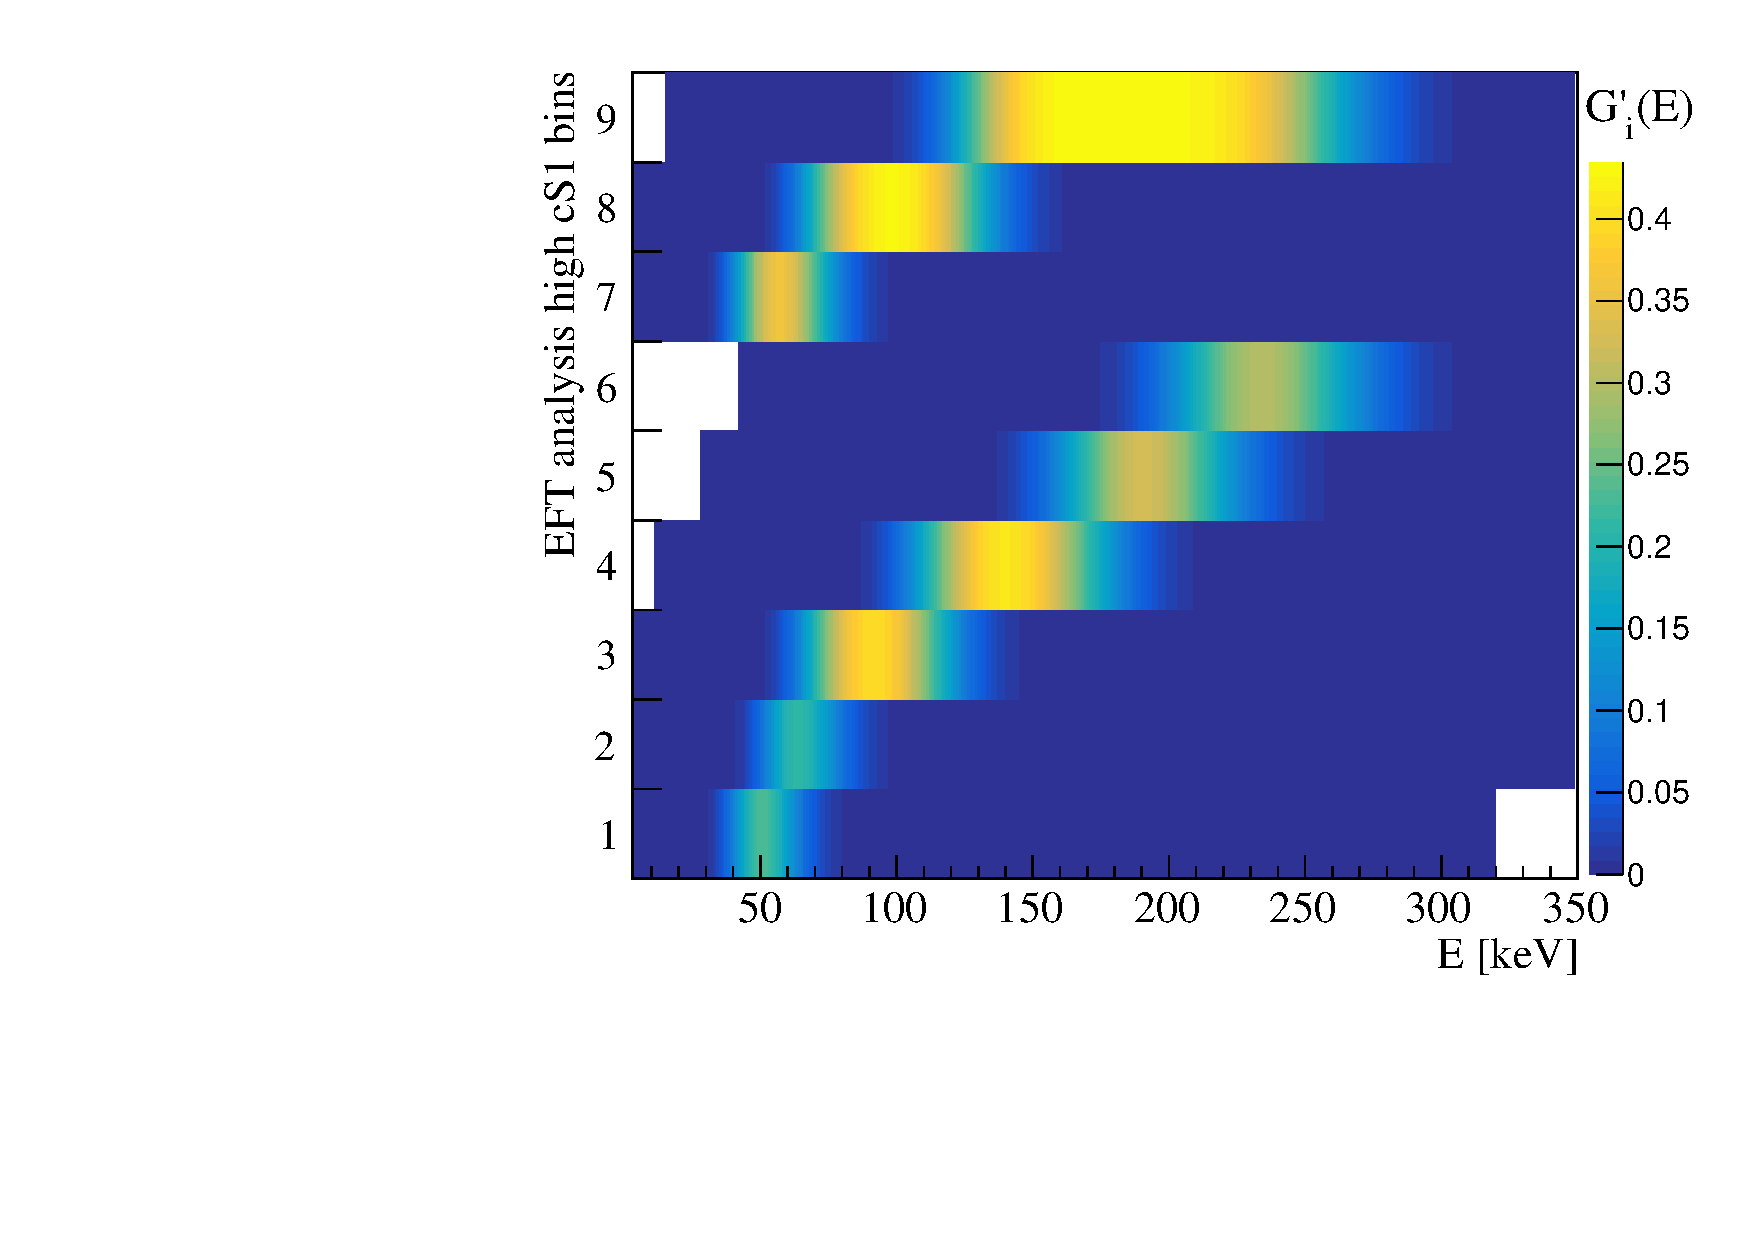
\includegraphics[width=1.\linewidth]{Figures/smeartable_highE}}
\caption{A visualization of the detector response table for $-1\sigma$ (i.e. conservative) $\Leff$, as provided in the supplementary material. The y axis indicates the bins used for the high-energy signal region of this analysis (explained in ~\ref{table:BinDef}). The $x$ axis shows recoil energies, and the colors give the probability density for a recoil of a given recoil energy to produce an event in each analysis bin. To produce a signal model for this analysis, one simply multiplies the table values by $\mathrm{d}R/\mathrm{d}E$ and integrates over $E$. The result is the predicted signal rate for each analysis bin.}
\label{fig:smeartable_highE}
\end{figure}  

\begin{table}
{
  \lstset{tabsize=4,basicstyle=\tiny\ttfamily,columns=flexible,emptylines=10000,keepspaces=true}
  \lstinputlisting{smeartable_Leff-1.dat}
}
\caption{Detector response table using $\Leff$ with constrained scaling parameter set to $-1\sigma$ value. First column gives recoil energies, subsequent columns give the values of $G'_i(E)$ for each of the 9 high-energy analysis bins. The sampling is in steps of $10~\keVr$, which is too coarse to give an accurate signal model for very low WIMP masses, but is suitable for the mass range most relevant to our analysis. Higher resolution $G'_i(E)$ functions, and $G'_i(E)$ functions for other values of $\Leff$, are given in supplementary material. 
\label{tab:smeartable_highE}
}
\end{table}  
\newpage
\subsection{Example code}
\label{app:example_code}
\begin{lstlisting}
import numpy as np
from numpy import newaxis
from scipy.interpolate import interp1d

def TrapI(x,y):
    """Simple trapezoid integration"""
    w = x[1:] - x[:-1]
    h = (y[1:] + y[:-1])/2.
    return np.sum(w*h,axis=0)

# Load detector response table
data = np.loadtxt("detector_table.dat")
E = data[:,0]; Gi = data[:,1:]

# Load test recoil spectrum (1 TeV WIMP, O6)
data = np.loadtxt("O6_1TeV.dat")
Er = data[:,0]
# Input spectra is normalised to coupling^2=1,
# rescale to something near limit (1e3)
# Also multiply in the appropriate exposure
dRdE = data[:,1] * (1e3/1.) * 224.6*34.
# Interpolate recoil spectrum to table values
# Assume spectrum zero outside data given
f_dRdE = interp1d(Er,dRdE)
dRdE_matched = f_dRdE(E)
Ri = TrapI(E[:,newaxis],Gi*dRdE_matched[:,newaxis])

for i,R in enumerate(Ri):
  print "bin {0}: rate = {1:.2g}".format(i+1,R)

Output:

bin 1: rate = 0.081
bin 2: rate = 0.098
bin 3: rate = 0.35
bin 4: rate = 0.46
bin 5: rate = 0.29
bin 6: rate = 0.22
bin 7: rate = 0.18
bin 8: rate = 0.47
bin 9: rate = 0.84
\end{lstlisting}

%\vfill

